\documentclass{article}
\usepackage{amsmath}
%%
%% Default settings for artisynth
%%
\NeedsTeXFormat{LaTeX2e}
%%\ProvidesPackage{artisynthDoc}[2012/04/05]

\usepackage[T1]{fontenc}
\usepackage[latin1]{inputenc}
\usepackage{listings}
\usepackage{makeidx}
\usepackage{latexml}
\usepackage{graphicx}
\usepackage{framed}
\usepackage{color}

\newcommand{\pubdate}{\today}
\newcommand{\setpubdate}[1]{\renewcommand{\pubdate}{#1}}

\iflatexml
\usepackage{hyperref}
\else
%% then we are making a PDF, so include things that LaTeXML can't handle: 
%% docbook style, \RaggedRight
\usepackage{ifxetex}
\usepackage{pslatex} % fixes fonts; in particular sets a better-fitting \tt font

\usepackage[A4]{artisynth_papersize}
%\usepackage[letter]{artisynth_papersize}
\usepackage[hyperlink]{asciidoc-dblatex} 

%\usepackage{verbatim}
\usepackage{ragged2e}
\setlength{\RaggedRightRightskip}{0pt plus 4em}
\RaggedRight
\renewcommand{\DBKpubdate}{\pubdate}
\renewcommand{\DBKreleaseinfo}{}
\fi

% set hypertext links to be dark blue:
\definecolor{darkblue}{rgb}{0,0,0.8}
\definecolor{sidebar}{rgb}{0.5,0.5,0.7}
\hypersetup{colorlinks=true,urlcolor=darkblue,linkcolor=darkblue}

%%%%%%%%%%%%%%%%%%%%%%%%%%%%%%%%%%%%%%%%%%%%%%%%%%%%%%%%%%%%%%%%%%%%%%%%%%%%%
%
% Define macros for handling javadoc class and method references
%
%%%%%%%%%%%%%%%%%%%%%%%%%%%%%%%%%%%%%%%%%%%%%%%%%%%%%%%%%%%%%%%%%%%%%%%%%%%%%
\makeatletter

% code inspired by http://stackoverflow.com/questions/2457780/latex-apply-an-operation-to-every-character-in-a-string
\def\removeargs #1{\doremoveargs#1$\wholeString\unskip}
\def\doremoveargs#1#2\wholeString{\if#1$%
\else\if#1({()}\else{#1}\taketherest#2\fi\fi}
\def\taketherest#1\fi
{\fi \doremoveargs#1\wholeString}

% Note: still doesn't work properly when called on macro output ...
% i.e., \dottoslash{\concatnames{model}{base}{foo}} fails 
\def\dottoslash #1{\dodottoslash#1$\wholeString\unskip}
\def\dodottoslash#1#2\wholeString{\if#1$%
\else\if#1.{/}\else{#1}\fi\dottaketherest#2\fi}
\def\dottaketherest#1\fi{\fi \dodottoslash#1\wholeString}

% concatenates up to three class/method names together, adding '.' characters
% between them. The first and/or second argument may be empty, in which case
% the '.' is omitted. To check to see if these arguments are empty, we
% use a contruction '\if#1@@', which will return true iff #1 is empty
% (on the assumption that #1 will not contain a '@' character).
\def\concatnames
#1#2#3{\if#1@@\if#2@@#3\else #2.#3\fi\else\if#2@@#1.#3\else#1.#2.#3\fi\fi}

\newcommand{\javabase}{}
\newcommand{\setjavabase}[1]{\renewcommand{\javabase}{#1}}

\iflatexml
\newcommand{\javaclassx}[2][]{%
% Includes code to prevent an extra '.' at the front if #1 is empty. It
% works like this: if '#1' is empty, then '#1.' expands to '.', and so 
% '\if#1..' will return true, in which case we just output '#2'.
\href{@JDOCBEGIN/\concatnames{\javabase}{#1}{#2}@JDOCEND}{#2}}
\newcommand{\javaclass}[2][]{%
\href{@JDOCBEGIN/\concatnames{}{#1}{#2}@JDOCEND}{#2}}

\newcommand{\javamethodArgsx}[2][]{%
\href{@JDOCBEGIN/\concatnames{\javabase}{#1}{#2}@JDOCEND}{#2}}
\newcommand{\javamethodArgs}[2][]{%
\href{@JDOCBEGIN/\concatnames{}{#1}{#2}@JDOCEND}{#2}}
\newcommand{\javamethodAlt}[2]{%
\href{@JDOCBEGIN/\concatnames{}{}{#1}@JDOCEND}{#2}}
\newcommand{\javamethodAltx}[2]{%
\href{@JDOCBEGIN/\concatnames{\javabase}{}{#1}@JDOCEND}{#2}}

\newcommand{\javamethodNoArgsx}[2][]{%
\href{@JDOCBEGIN/\concatnames{\javabase}{#1}{#2}@JDOCEND}{\removeargs{#2}}}
\newcommand{\javamethodNoArgs}[2][]{%
\href{@JDOCBEGIN/\concatnames{}{#1}{#2}@JDOCEND}{\removeargs{#2}}}
\else
\def\javaurl{http://www.artisynth.org/doc/javadocs/}
\newcommand{\javaclassx}[2][]{{\color{darkblue}#2}}
%\href{\javaurl\dottoslash{\concatnames{\javabase}{#1}{#2}}.html}{#2}}
\newcommand{\javamethodArgsx}[2][]{{\color{darkblue}#2}}
\newcommand{\javamethodNoArgsx}[2][]{{\color{darkblue}\removeargs{#2}}}
\newcommand{\javaclass}[2][]{{\color{darkblue}#2}}
%\href{\javaurl\dottoslash{\concatnames{\javabase}{#1}{#2}}.html}{#2}}
\newcommand{\javamethodArgs}[2][]{{\color{darkblue}#2}}
\newcommand{\javamethodNoArgs}[2][]{{\color{darkblue}\removeargs{#2}}}
\newcommand{\javamethodAlt}[2]{{\color{darkblue}{#2}}}
\newcommand{\javamethodAltx}[2]{{\color{darkblue}{#2}}}
\fi

\newcommand{\javamethod}{\@ifstar\javamethodNoArgs\javamethodArgs}
\newcommand{\javamethodx}{\@ifstar\javamethodNoArgsx\javamethodArgsx}

%%%%%%%%%%%%%%%%%%%%%%%%%%%%%%%%%%%%%%%%%%%%%%%%%%%%%%%%%%%%%%%%%%%%%%%%%%%%%
%
% Define macros for sidebars
%
%%%%%%%%%%%%%%%%%%%%%%%%%%%%%%%%%%%%%%%%%%%%%%%%%%%%%%%%%%%%%%%%%%%%%%%%%%%%%

\iflatexml
\newenvironment{sideblock}{\begin{quote}}{\end{quote}}
\else
\usepackage[strict]{changepage}
\definecolor{sidebarshade}{rgb}{1.0,0.97,0.8}
\newenvironment{sideblock}{%
    \def\FrameCommand{%
    \hspace{1pt}%
    {\color{sidebar}\vrule width 2pt}%
    %{\vrule width 2pt}%
    {\color{sidebarshade}\vrule width 4pt}%
    \colorbox{sidebarshade}%
  }%
  \MakeFramed{\advance\hsize-\width\FrameRestore}%
  \noindent\hspace{-4.55pt}% disable indenting first paragraph
  \begin{adjustwidth}{}{7pt}%
  %\vspace{2pt}\vspace{2pt}%
}
{%
  \vspace{2pt}\end{adjustwidth}\endMakeFramed%
}
\fi

\iflatexml
\newenvironment{shadedregion}{%
  \definecolor{shadecolor}{rgb}{0.96,0.96,0.98}%
  \begin{shaded*}%
% Put text inside a quote to create a surrounding blockquote that
% will properly accept the color and padding attributes
  \begin{quote}%
}
{%
  \end{quote}%
  \end{shaded*}%
}
\else
\newenvironment{shadedregion}{%
  \definecolor{shadecolor}{rgb}{0.96,0.96,0.98}%
  \begin{shaded*}%
}
{%
  \end{shaded*}%
}
\fi

% Wanted to create a 'listing' environment because lstlisting is
% tedious to type and because under latexml it may need
% some massaging to get it to work properly. But hard to do
% because of the verbatim nature of listing
%\iflatexml
%\newenvironment{listing}{\begin{lstlisting}}{\end{lstlisting}}%
%\else
%\newenvironment{listing}{\begin{lstlisting}}{\end{lstlisting}}%
%\fi

\iflatexml\else
% fancyhdr was complaining that it wanted a 36pt header height ...
\setlength{\headheight}{36pt}
\fi

% abbreviation for backslash character
\newcommand\BKS{\textbackslash}


% Convenience stuff
\newcommand{\ifLaTeXMLelse}[2]{%
  \iflatexml %
  #1 %
  \else %
  #2 %
  \fi %
}

\newcommand{\ifLaTeXML}[1]{ %
  \iflatexml %
  #1 %
  \fi %
}

\makeatother


\setcounter{tocdepth}{5}
\setcounter{secnumdepth}{3}

\title{Writing Documentation for ArtiSynth}
\author{John Lloyd}
\setpubdate{Last updated: April, 2018}
\iflatexml
\date{}
\fi

\begin{document}

\maketitle

\iflatexml{\large\pubdate}\fi

\tableofcontents

\section{Introduction}

This document describes how to write and modify the main ArtiSynth
documentation set. It explains where the documentation sources are
kept, how they are converted into HTML or PDF files, what external
software is required, and what special conventions are used.

In addition to the main documentation described here, there may be
additional documentation available at
\href{http://www.artisynth.org}{www.artisynth.org}.

\section{How Documents Are Created}

ArtiSynth documentation is written using LaTeX, and converted into
either PDF files, single HTML files for direct browser viewing, or
sectioned HTML files for viewing within an Eclipse InfoCenter (Section
\ref{InfoCenterSec}). PDF files are built using {\tt latex}, {\tt
dvips} and {\tt eps2pdf} as described in Section
\ref{BuildingPDFSec}. Single and sectioned HTML files are built
using LaTeXML
(\href{http://dlmf.nist.gov/LaTeXML/}{dlmf.nist.gov/LaTeXML}), as
described in Sections \ref{BuildingSingleHTMLSec} and \ref{BuildingSectionedHTMLSec}.

{\tt Makefile}s are used to organize the commands and options needed
to build these different outputs. As such, documentation is most
easily built on systems that support {\it GNU make}, such as
Linux, MacOS, or Windows running Cygwin or some other Unix-like shell.

The format for PDF output is based on that used by the
\href{http://www.docbook.org}{DocBook} project, while the style for
HTML files is based on that used by
\href{http://www.methods.co.nz/asciidoc}{AsciiDoc}.

\begin{sideblock}
The usual workflow when editing or changing an ArtiSynth document is:

- Edit the {\tt .tex} file in a text editor\\
- Run {\tt make html} and/or {\tt make pdf} to build HTML
or PDF files (Section \ref{DocumentCreationSec})\\
- If appropriate, run {\tt make install} to install the files on the
ArtiSynth webserver (Section \ref{InstallingSec})\\
- Examine the output using a browser or PDF reader
\end{sideblock}

\subsection{Document Source Code Organization}

The sources for the various books and articles that make up the
documentation are located in subdirectories in {\tt
<ARTISYNTH\_HOME>/doc}.  For example, the sources for this document
are located in {\tt <ARTISYNTH\_HOME>/doc/documentation}, and the
source file itself is called {\tt documentation.tex}. 
By convention, if a
document contains images, then its image files are stored in a
sub-directory called {\tt images}.

Additional subdirectories of {\tt doc} include:

\begin{description}

\item[{\tt misc/}] \mbox{}

Contains miscellaneous and older documentation, including
text files.

\item[{\tt javadocs/}] \mbox{}

Contains the Javadoc API documentation.

\item[{\tt html/}] \mbox{}

Contains the HTML output produced by LaTeXML.

\item[{\tt pdf/}] \mbox{}

Contains the PDF files.

\item[{\tt texinputs/}] \mbox{}

Contains input and style files used by LaTeX.

\item[{\tt style/}] \mbox{}

Contains CSS style sheets.

\end{description}

\subsection{Makefile commands to build documents}
\label{DocumentCreationSec}

Each documentation source directory contains a {\tt Makefile}, which
implements a few basic commands to build PDF and/or HTML output files
from the LaTeX source files.  To use the {\tt Makefile} commands, you
need to be on a system that supports {\it GNU make}. This includes
Linux, MacOS, and Windows with Cygwin installed.

\subsubsection{Javadocs}
\label{MakingJavadocsSec}

Java API documentation is built in the directory {\tt
<ARTISYNTH\_HOME>/doc/javadocs} by running the command
%
\begin{verbatim}
  > make javadocs
\end{verbatim}
%
from within the directory {\tt <ARTISYNTH\_HOME>/doc}.

\subsubsection{HTML files}
\label{MakingHTMLSec}

To build a single HTML file for a particular source document,
run the command
%
\begin{verbatim}
  > make html
\end{verbatim}
%
within that document's source directory. This will build the HTML
file, as described in Section \ref{BuildingSingleHTMLSec}, and place it
in a subdirectory under {\tt <ARTISYNTH\_HOME>/doc/html}. It will also
copy over any required image files.

\begin{sideblock}
If the documentation contains Javadoc API references, using the {\tt
\BKS javaclass} or {\tt \BKS javamethod} commands described in Section
\ref{JavadocRefsSec}, then it is necessary to ensure that the Javadocs
are built and up-to-date (Section
\ref{MakingJavadocsSec}). Otherwise, links to the specified Javadocs
may not be found, resulting in warning messages that look like
%
\begin{verbatim}
...
WARNING: class maspack.properties.HasProperties not found
Can't open ../javadocs/maspack/properties/HasProperties.html: No such file or directory
WARNING: class maspack.properties.HasProperties not found for method getProperty
WARNING: class maspack.properties.Property not found
...
\end{verbatim}
%
\end{sideblock}

To build subsectioned HTML files for a viewing a source document
within an Eclipse InfoCenter, run the command
%
\begin{verbatim}
  > make infocenter
\end{verbatim}
%
This will build HTML files for the document subsections, along with
a table of contents for use by {\tt InfoCenter}, as described
in Section \ref{BuildingSectionedHTMLSec},
and place them in
a subdirectory under {\tt <ARTISYNTH\_HOME>/doc/html}.  The table of
contents file is an XML file and will generally have the name {\tt
<document>Toc.xml}, where {\tt <document>} is the base name of the
source document.

To build single or sectioned HTML files for {\it all} the
documentation, you can run the commands
%
\begin{verbatim}
  > make HTML
\end{verbatim}
%
or
%
\begin{verbatim}
  > make INFOCENTER
\end{verbatim}
%
from within the documentation root directory {\tt
<ARTISYNTH\_HOME>/doc}.

\subsubsection{PDF files}
\label{MakingPDFSec}

To build a PDF file for a document, you can use the command
%
\begin{verbatim}
  > make pdf
\end{verbatim}
%
within that document's source directory. This will build a PDF file,
as described in Section \ref{BuildingPDFSec}, and copy it into the directory 
{\tt <ARTISYNTH\_HOME>/doc/pdf}.

To build PDF files for {\it all} the documentation, you can run the
command
%
\begin{verbatim}
  > make PDF
\end{verbatim}
%
from within the documentation root directory {\tt
<ARTISYNTH\_HOME>/doc}.

\subsubsection{Other Commands}

Within a document's directory, the simple command
%
\begin{verbatim}
  > make
\end{verbatim}
%
will build both HTML {\it and} PDF output files.

By way the {\tt make} operates, output will usually only be built when
the output file does not exist or when it's older than the
corresponding {\tt .tex} source file. To ensure execution of a particular
{\tt make} command within a document's source directory,
you can precede it with
%
\begin{verbatim}
  > make clean
\end{verbatim}
%
which will remove all extraneous and output files. Likewise,
to clean {\it all} documents, you can run 
%
\begin{verbatim}
  > make CLEAN
\end{verbatim}
%
from within the documentation root directory {\tt <ARTISYNTH\_HOME>/doc}.

Finally, the command
%
\begin{verbatim}
  > make all
\end{verbatim}
%
from within the documentation root directory, is
equivalent to 
%
\begin{verbatim}
  > make javadocs PDF HTML INFOCENTER
\end{verbatim}
%

\subsection{Building single HTML files}
\label{BuildingSingleHTMLSec}

A single HTML file for a document is built
using LaTeXML (Section \ref{InstallingLaTeXMLSec}), plus some
additional post-processing. For a document file {\tt
document.tex}, located in the source directory {\tt
<ARTISYNTH\_HOME>/doc/document}, a typical command sequence 
executed from within the source directory would look like this:

\begin{lstlisting}[]
  latexml document.tex > document.xml
  latexmlpost --mathimages --format=html4 --css=../style/artisynth.css \
     --destinatiom=../html/document/document.html
  postprocessLatexml --jdocDir ../javadocs --jdocUrl ../../javadocs \
     --docBase .. ../html/document/document.html
\end{lstlisting}

{\tt latexml} and {\tt latexmlpost} are both commands supplied with
LaTeXML. The former converts LaTeX input into an XML file, which the
latter then converts into HTML, with the result being placed into {\tt
<ARTISYNTH\_HOME>/doc/html/document/document.html}.

The command {\tt postprocessLatexml} is a script defined in {\tt
<ARTISYNTH\_HOME>/bin} which does further post-processing on the HTML
file. It does this by invoking two Perl scripts, {\tt setJavadocLinks}
and {\tt fixLatexmlOuput}, described in detail in Section
\ref{LocalCustomizationSec}, which correctly set URL links to other
parts of the documentation and fix some minor issues with the HTML
produced by LaTeXML. The arguments {\tt \DHY jdocDir}, {\tt \DHY jdocUrl}
and {\tt \DHY docBase} are passed directly to {\tt setJavadocLinks}.

\subsection{Building sectioned HTML files}
\label{BuildingSectionedHTMLSec}

For use with InfoCenter (Section \ref{InfoCenterSec}), the HTML output
for a document needs to be split into multiple files corresponding to
different chapters and sections. This is done with LaTeXML, using a
command sequence similar to that described in
Section \ref{BuildingSingleHTMLSec}:

\begin{lstlisting}[]
  latexml document.tex > document.xml
  latexmlpost --mathimages --format=html4 --css=../style/artisynth.css \
     --splitat=section --destinatiom=../html/document/document.html
  postprocessLatexml --jdocDir ../javadocs --jdocUrl ../../javadocs \
     --docBase https://www.artisynth.org/doc/info ../html/document/*.html
\end{lstlisting}

The main differences are the {\tt \DHY splitat=section} option to {\tt
latexmlpost}, causing the HTML to be split into multiple files at the
section level, and, for {\tt postprocessLatexml}, the specification of
{\tt \DHY docBase} as\\ {\tt https://www.artisynth.org/doc/info},
which will cause references to other manuals to be routed through the
InfoCenter URL.

InfoCenter also requires an XML file describing the document's table
contents. This is generated from the file {\tt documentToc.html}
(produced by {\tt latexmlpost}), using the standalone Java program
%
\begin{verbatim}
  artisynth.core.util.BuildInfoCenterToc
\end{verbatim}
%

\subsection{Building PDF files}
\label{BuildingPDFSec}

A PDF file for a document is built using {\tt latex}, {\tt dvips},
some PostScript post-processing, and {\tt ps2pdf}. For a document file
{\tt document.tex}, located in the source directory {\tt
<ARTISYNTH\_HOME>/doc/document}, a typical command sequence executed
from within the source directory would look like this:

\begin{lstlisting}[]
  latex document.tex
  latex document.tex
  dvips -j0 document
  setJavadocLinks --postscript --out tmpfile.ps --jdocDir ../javadocs \
     --jdocUrl https://www.artisynth.org/doc/javadocs --docBase doc/pdf document.ps
  mv tmpfile.ps document.ps
  ps2pdf document.ps
\end{lstlisting}

{\tt latex} is called twice to resolve references, and then {\tt
dvips} converts the DVI file into PostScript. The {\tt -j0} option is
passed to {\tt dvips} because partial font loading sometimes causes
missing letters in fonts embedded image files.  After the PostScript
is produced, it is postprocessed by the Perl script {\tt
setJavadocLinks} (Section \ref{setJavadocLinksSec}) to correctly set
URL links to other parts of the documentation. The modified PostScript
is then converted to PDF using {\tt ps2pdf}.

\begin{sideblock}
The reason for converting LaTeX to PostScript, instead of PDF directly, is because
{\tt setJavadocLinks} does not work on PDF files.
\end{sideblock}

\subsection{Installing Documents on the Webserver}
\label{InstallingSec}

Once you have built the documentation, you may wish to install it on the
ArtiSynth webserver. In order to do this, you need

\begin{enumerate}
\item An account on the ArtiSynth webserver (which is currently {\tt
research.hct.ece.ubc.ca}). To ensure proper file access, this account
should be a member of the group {\tt www-data}.
\item The environment variable {\tt ARTISYNTH\_WEB\_ACCOUNT} set to
your username on that server, {\it if} that username is different
from the username on your local machine.
\item {\tt ssh} and {\tt rsync} installed on your local machine.
\end{enumerate}

Then, from within a given documentation subdirectory, the {\tt make}
command
%
\begin {verbatim}
  > make install_html
\end{verbatim}
%
will build all the HTML output associated with that directory and install
it on the ArtiSynth webserver. Likewise, the command
%
\begin {verbatim}
  > make install_pdf
\end{verbatim}
%
will build and install the PDF output, and
%
\begin {verbatim}
  > make install
\end{verbatim}
%
will install both HTML and PDF.

From the main documentation directory {\tt <ARTISYNTH\_HOME>/doc}, you
can build and install {\it all} the HTML and PDF documentation with
the command
%
\begin{verbatim}
  > make install
\end{verbatim}
%
HTML and PDF can also be built and installed separately with the
individual commands
%
\begin {verbatim}
  > make install_html
  > make install_pdf
\end{verbatim}
%
Also, from within {\tt <ARTISYNTH\_HOME>/doc}, the command
%
\begin{verbatim}
  > make install_javadocs
\end{verbatim}
%
will install the Javadocs. Note that {\tt install\_javadocs} assumes
you have already built the Javadocs, which as described above you can
do using the command
%
\begin{verbatim}
  > make javadocs
\end{verbatim}
%
\begin{sideblock}
All of these installation commands work by using {\tt rsync}
to copy the files and
{\tt ssh} to then correctly set the permissions of the copied files.
If you don't have an SSH key arranged between your local machine
and the webserver, this will generally require 
you to enter a password twice.
\end{sideblock}

\section{LaTeX usage and conventions}

\label{LatexUsage}

\subsection{LaTeXML restrictions}

All documentation is written in LaTeX, and conversion to HTML is done
using \href{http://dlmf.nist.gov/LaTeXML/}{LaTeXML} (Section
\ref{InstallingLaTeXMLSec}).  Currently, version 0.8.0 or higher of
LaTeXML is required; see Section \ref{ExternalSoftwareSec}.

LaTeXML supports many, but not all, of the commonly used LaTeX
packages. Therefore, in some circumstance, it may be useful to
conditionalize the LaTeX source to use different input depending on
whether HTML or PDF output is being produced. Producing HTML implies
the use of LaTeXML, which can be detected using the {\tt \BKS
iflatexml} conditional, as in:

\begin{lstlisting}[]
\iflatexml
  do things in a conventional way that LaTeXML can deal with
\else
  \fancydancy{use some LaTeX package that LaTeXML can't handle}
\fi
\end{lstlisting}

Some specific problems with LaTeXML at the time of this writing
include:

\begin{itemize}

\item For item entries within a description list ( {\tt \BKS
begin\{description\} ... \BKS end\{description\}}), it may sometimes
be necessary to add a {\tt \BKS mbox\{\}} macro after the item
label, as in
\begin{verbatim}
  \item[labelForItem]\mbox{}
\end{verbatim}
in order to ensure that the text following the label starts on a new
line.

\item LaTeXML does not place the title page date (specified using {\tt
\BKS date\{\}}) on the titlepage. Instead, it is placed in the
footer at the page bottom. As a work-around, we use {\tt \BKS iflatex} to
leave {\tt \BKS date} empty and then place an explicit date at the top of
the page.

\item In some earlier versions of LaTeXML, blank lines were not
properly handled in the {\tt lstlisting} environment. This was fixed by
post-processing the HTML output, as described in Section
\ref{fixLatexmlOutputSec}.

\item In some cases, the first line in a {\tt lstlisting} environment
may not appear, unless a {\tt []} is appended to the opening \\
{\tt \BKS begin\{lstlisting\}}, as in
%
\begin{verbatim}
  \begin{lstlisting}[]
  ... verbatim listing ...
  \end{lstlisting}
\end{verbatim}
%

\item Some characters and character sequences (such as quotes, and the
sequence {\tt ...}) are converted into special unicode characters.
This actually reduces the readability of code blocks, and so
post-processing is used to replace the unicode characters with the
originals (Section \ref{fixLatexmlOutputSec}).

\end{itemize}

\subsection{Font conventions}

Programmatic literals, such as class and method names, file names, 
command sequences, and
environment variables are typeset in {\tt monospace}, using {\tt
\{\BKS tt monospace\}}. User interface literals, such as menu items, are
typeset in {\sf sans-serif}, using {\tt \{\BKS sf sans-serif\}}.

\subsection{Code blocks}

Small code blocks (typically one-line) are usually typeset using the
{\tt verbatim} environment, which produces output like this:

\begin{verbatim}
  > short one line code or command line example
\end{verbatim}

Longer code examples are typeset using the {\tt lstlisting}
environment (from the {\tt listings} package), which surrounds
the output in a colored box:

\begin{lstlisting}[]
// Here is a longer code example
interface Property
{
   Object get(); 
   void set (Object value); 
   Range getRange ();
   HasProperties getHost();
   PropertyInfo getInfo();
}
\end{lstlisting}

\subsection{Side blocks}
\label{SideBlocksSec}

A special environment called {\tt sideblock} is used to create
admonition sections that contain special notes, warnings, or side
information. The LaTeX source

\begin{lstlisting}[]
\begin{sideblock}
Note: when producing PDF, the {\tt sideblock} environment
is implemented using commands from the {\tt color} and
{\tt framed} packages. When producing HTML output, side blocks
are implemented internally using the
regular {\tt quote} environment, with the final appearance arranged
using the CSS stylesheet. 
\end{sideblock}
\end{lstlisting}

will produce output that looks like this:

\begin{sideblock}
Note: when producing PDF, the {\tt sideblock} environment
is implemented using commands from the {\tt color} and
{\tt framed} packages. When producing HTML output, side blocks
are implemented internally using the
regular {\tt quote} environment, with the final appearance arranged
using the CSS stylesheet. 
\end{sideblock}

\subsection{Inserting Images}
\label{InsertingImagesSec}

Image files are input using {\tt \BKS includegraphics} from the {\tt
graphics} package, using code fragments of the form
%
\begin{lstlisting}[]
\begin{figure}
\begin{center}
  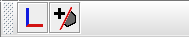
\includegraphics[]{images/viewerToolbar}
\end{center}
\caption{The viewer toolbar.}%
\end{lstlisting}
%
When specifying the image file (e.g., {\tt images/viewerToolbar} in
the above example), the file extension is typically omitted, allowing
the processing application ({\tt LaTeXML} for HTML and {\tt latex} for
PDF) to determine the appropriate file type.  {\tt LaTeXML} generally
requires {\tt .png}, {\tt .jpg}, {\tt .pdf} or {\tt .eps}
(encapsulated PostScript) files, whereas {\tt latex}, because we are
using it to first create PostScript, is constrained to
encapsulated PostScript ({\tt .eps}). The {\tt Makefile}s
provide default rules for creating {\tt .eps} files; see Section
\ref{ImagesSec} for details.

Our convention is to store image files in a subdirectory {\tt images}
of the documentation source directory. When building HTML output,
these are copied automatically into the appropriate HTML target directory.

In some cases, good image appearance may require different image
scalings, depending on whether HTML or PDF output is being
produced. This is often true in particular for {\tt .png} files, where
for HTML one may not want any scaling at all (in order to get
pixel-for-pixel reproduction). This can be achieved using
{\tt \BKS iflatexml}:

\begin{lstlisting}[]
\begin{figure}
\begin{center}
  \iflatexml
    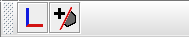
\includegraphics[]{images/viewerToolbar}
  \else
    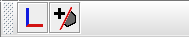
\includegraphics[width=2.5in]{images/viewerToolbar}
  \fi
\end{center}
\caption{The viewer toolbar.}%
\end{lstlisting}

\subsection{Javadoc References}
\label{JavadocRefsSec}

ArtiSynth is implemented in Java, and so much of the documentation
refers to various Java classes and methods. It is therefore useful to
include hyperlinks from the documentation to the actual Javadoc pages.
Unfortunately, creating such a hyperlink can be rather tedious: If the
Javadocs are rooted at {\tt http://www.artisynth.org/doc/javadocs},
then a hyperlink to the class definition for {\tt
maspack.matrix.MatrixNd} must take the lengthy form
\begin{verbatim}
  \href{http://www.artisynth.org/doc/javadocs/maspack/matrix/MatrixNd.html}{MatrixNd}
\end{verbatim}
Method references are even worse, particularly if they contain arguments:
\begin{verbatim}
  \href{http:// ... MatrixNd.html#mul(maspack.matrix.MatrixNd)}{MatrixNd.mul()}
\end{verbatim}
To alleviate these problems, several LaTeX commands are provided that
build Javadoc references automatically from simple class and
method descriptions.

\subsubsection{Class references}
\label{ClassRefsSec}

The command {\tt \BKS javaclass} will create a Javadoc reference to 
a class from the class name itself. The LaTeX source

\begin{lstlisting}[]
\javaclass{maspack.matrix.MatrixNd}, and \javaclass[maspack]{matrix.MatrixNd}, and
\javaclass[maspack.matrix]{MatrixNd}.
\end{lstlisting}

will produce the output

\javaclass{maspack.matrix.MatrixNd}, and \javaclass[maspack]{matrix.MatrixNd}, and
\javaclass[maspack.matrix]{MatrixNd}.

The name in the optional argument (between square brackets {\tt []})
is prepended to the main argument to create a fully qualified class name,
with only the main argument being used as the anchor text. 

The names provided by the optional argument and the main argument are
concatenated (with an intervening '{\tt .}' character) to create a
fully qualified class name that is used to produce the appropriate
hyperlink to the Javadoc. 

When referencing an inner class or enumerated type, one should
separate the subclass name from the main class name with an escaped
dollar sign {\tt \$} instead of a {\tt .} character. This allows {\tt \BKS
javaclass} to distinguish class name separators from package name
separators (which need to be converted to file separators). The
hash tags will be converted to dot characters on output.

For example, the LaTeX source 

\begin{lstlisting}[]
Use the \javaclass[maspack.matrix]{Matrix\$WriteFormat} to control formatting.
\end{lstlisting}

will produce the output:

Use the \javaclass[maspack.matrix]{Matrix\$WriteFormat} to control formatting.

Complete control over the anchor test can be
achieved using the {\tt \BKS javaclassAlt} macro, which takes two
arguments: the class reference, and the visible text. So for example,
the LaTeX source

\begin{lstlisting}[]
Use the \javaclassAlt{maspack.matrix.Matrix\$WriteFormat}{WriteFormat}
to control formatting.
\end{lstlisting}

will produce the output:

Use the \javaclassAlt{maspack.matrix.Matrix\$WriteFormat}{WriteFormat}
to control formatting.

{\tt \BKS javaclassAlt} is also useful in cases where one needs to
embed a {\tt \#} tag in the class reference, such as when referring to
fields of an enumerated type. The {\tt \#} tag can be placed
in the first argument, as in this example,

\begin{lstlisting}[]
\javaclassAlt{maspack.matrix.Matrix\$WriteFormat\#CRS}{WriteFormat.CRS} causes
the matrix to be written using the compressed row storage format.
\end{lstlisting}

which produces the output:

\javaclassAlt{maspack.matrix.Matrix\$WriteFormat\#CRS}{WriteFormat.CRS} causes
the matrix to be written using the compressed row storage format.

%For additional brevity in the LaTeX source
%file, one can also use the command {\tt \BKS javaclassx}, which
%internally prepends a package name provided by the expansion of {\tt
%\BKS javabase} onto the class name. {\tt \BKS javabase} can be set
%using the command {\tt \BKS setjavabase}, thus removing the need to
%explicly specify the full class name in the arguments to {\tt \BKS
%javaclassx}. For example,
%
%\begin{lstlisting}[]
%\setjavabase{maspack.matrix}
%Two important classes are \javaclassx{MatrixNd} and \javaclassx{VectorNd}.
%\end{lstlisting}
%
%will produce the output
%
%\setjavabase{maspack.matrix}
%Two important classes are \javaclassx{MatrixNd} and \javaclassx{VectorNd}.

\subsubsection{Method references}

Methods can be referenced in a similar way using the command {\tt
\BKS javamethod}, which takes a class name plus the name of a method and
a (possibly abbreviated) argument signature.
LaTeX source of the form

\begin{lstlisting}[]
\javamethod{maspack.matrix.MatrixNd.mul()}, 
\javamethod[maspack.matrix]{MatrixNd.mul(MatrixNd)},
\javamethod[maspack.matrix.MatrixNd]{mul(MatrixNd,MatrixNd)}.
\end{lstlisting}

will produce output of the form

\setjavabase{}
\javamethod{maspack.matrix.MatrixNd.mul()}, 
\javamethod[maspack.matrix]{MatrixNd.mul(MatrixNd)},
\javamethod[maspack.matrix.MatrixNd]{mul(MatrixNd,MatrixNd)}.

%As with {\tt \BKS javaclass}, an alternate method {\tt \BKS
%javamethodx} is available which internally prepends the package name
%provided by the expansion of {\tt \BKS javabase} onto the class name,
%so that
%
%\begin{lstlisting}[]
%\setjavabase{maspack.matrix}
%\javamethodx[MatrixNd]{mul(MatrixNd)} takes one argument,
%while \javamethodx[MatrixNd]{mul(MatrixNd,MatrixNd)} takes two.
%\end{lstlisting}
%
%will produce output of the form
%
%\setjavabase{maspack.matrix}
%\javamethodx[MatrixNd]{mul(MatrixNd)} takes one argument,
%while \javamethodx[MatrixNd]{mul(MatrixNd,MatrixNd)} takes two.

The argument signature does not need to contain the fully qualified
type names of the arguments. In fact, if the method name is unique to
the class, no argument list is needed at all; a simple {\tt ()} will
suffice.  Otherwise, if the method is overloaded, the argument
signature should be composed of comma-separated entries, each of which
partly matches the fully qualified type name of each argument.

For example,

\begin{lstlisting}[]
\javamethod[maspack.matrix]{MatrixNd.mul(maspack.matrix.MatrixNd,maspack.matrix.MatrixNd)}, 
\javamethod[maspack.matrix]{MatrixNd.mul(matrix.MatrixNd,matrix.MatrixNd)},
\javamethod[maspack.matrix]{MatrixNd.mul(MatrixNd,MatrixNd)}.
\end{lstlisting}

will all produce references to the same method. In fact, if the method
name and argument count is unique, then a set of commas indicating the
number of arguments will be sufficient, as in {\tt
\BKS javamethod{MatrixNd.mul(,)}}.

To omit the argument signature from
the anchor text, one can use the alternate command {\tt \BKS javamethod*}
instead, so that

\begin{lstlisting}[]
Method reference with argument signature:
\javamethod[maspack.matrix]{MatrixNd.mul(MatrixNd,MatrixNd)}, and without:
\javamethod*[maspack.matrix]{MatrixNd.mul(MatrixNd,MatrixNd)}.
\end{lstlisting}

will produce the output

Method reference with argument signature:
\javamethod[maspack.matrix]{MatrixNd.mul(MatrixNd,MatrixNd)}, and without:
\javamethod*[maspack.matrix]{MatrixNd.mul(MatrixNd,MatrixNd)}.

Finally, one may sometimes want complete control over the visible text
associated with a method reference. For example,
instead of \javamethod[maspack.matrix]{MatrixNd.mul(MatrixNd,MatrixNd)},
one may wish to use 
\javamethodAlt{maspack.matrix.MatrixNd.mul(MatrixNd,MatrixNd)}%
{MatrixNd.mul(M1,M2)}. One can do this using the command
{\tt javamethodAlt}, which requires two arguments (and does
not take an optional argument):
%
\begin{lstlisting}[]
\javamethodAlt{maspack.matrix.MatrixNd.mul(MatrixNd,MatrixNd)}{MatrixNd.mul(M1,M2)}
\end{lstlisting}
%
The first argument specifies the class, method and arguments in enough
detail to locate the link, and the second specifies the visible text.

\subsubsection{How it works}
\label{HowJavadocLinksWorkSec}

{\tt \BKS javaclass} and {\tt \BKS javamethod} both work by creating a call
to {\tt \BKS href} with a placeholder link of the form

\begin{quote}
@{\tt JDOCBEGIN/<classOrMethodName>}@{\tt JDOCEND}
\end{quote}

This propagates to the output HTML or PostScript file, which is then
processed by the Perl script {\tt setJavadocLinks}, as described
in Section \ref{setJavadocLinksSec}, to set the correct URL.

\subsection{References to other ArtiSynth documents}

Within a given document, one may sometimes wish to provide a link to another
ArtiSynth document, such as the
\artisynthManual{maspack}{Maspack Reference Manual}. 
This can be done using the macro {\tt \BKS artisynthManual},
for which the above reference to the Maspack manual was 
encoded as follows:
%
\begin{lstlisting}[]
  \artisynthManual{maspack}{Maspack Reference Manual}
\end{lstlisting}
%
More generally, the macro takes the form
%
\begin{lstlisting}[]
  \artisynthManual[docpath]{docname}{text}
\end{lstlisting}
%
where {\tt docname} is the root name of the document (e.g., {\tt
maspack} for {\tt maspack.tex}), {\tt docpath} is an optional argument
giving the name of the directory containing the document, relative to
{\tt <ARTISYNTH\_HOME>/doc}, and {\tt text} is the text associated
with the hyperlink. If omitted, {\tt docpath} is assumed to be the
same as {\tt docname}.

Internally, {\tt \BKS artisynthManual} works by creating a placeholder
link containing the symbol @{\tt ARTISYNTHDOCBASE}. This propagates to
the output HTML or PostScript file, which is then processed by {\tt
setJavadocLinks} as described in Section \ref{setJavadocLinksSec}.

\section{Adding a New Document}

If you're adding a completely new document (as opposed
to modifying an existing one), then you should create a
new source directory for that document under {\tt <ARTISYNTH\_HOME>/doc},
and place the relevant {\tt .tex} files there.

\subsection{Creating and Updating the Makefiles}

You should also create a {\tt Makefile} in the new directory. This is most
easily done by copying an existing {\tt Makefile} from a similar document,
and replacing the names of the source files. 
Note that many of the commands
and variables are predefined in the file {\tt Makedefs}, included from
{\tt <ARTISYNTH\_HOME>/doc}.

You should also update the {\tt Makefile} in {\tt <ARTISYNTH\_HOME>/doc},
so that it is aware of the new document subdirectory. Most
likely this will just require adding the name of the new source
directory to the variable {\tt SUBDIRS}.

\subsection{Updating the InfoCenter}

Adding a new document will also require updating the configuration for
the InfoCenter (Section \ref{InfoCenterSec}), so that the InfoCenter
knows about it and can add it to its table of contents. See the
section ``Adding a New Document'' in the file
\begin{verbatim}
  <ARTISYNTH_HOME>/doc/INFOCENTER_README
\end{verbatim}

\subsection{Updating the ArtiSynth website}

The ArtiSynth website provides links to the various manuals and guides
(including PDF, HTML, and InfoCenter). These should be updated to
provide links to any new documentation, particularly on the main
documentation page at
\href{https://www.artisynth.org/doc}{www.artisynth.org/doc}.

\section{Images, IDraw and Xfig}
\label{ImagesSec}

As mentioned in Section \ref{InsertingImagesSec}, LaTeXML generally
requires image files of type {\tt .png}, {\tt .jpg}, {\tt .pdf} or
{\tt .eps} (encapsulated PostScript), while 
{\tt latex} requires image files of type {\tt .eps}. 
The {\tt Makefile}s provide default commands to automatically
create {\tt .eps} files on demand from {\tt .png}, {\tt .jpg}, or {\tt
.pdf} files, using the ImageMagick {\tt convert} program. 

A number of document illustrations are produced using the Interviews
IDraw graphics application, and stored as {\tt .idr} files. A default
Makefile command automatically converts these to {\tt .eps} (by a
simple copy operation since {\tt .idr} files are themselves
encapsulated PostScript).

In addition to raw image files, the Linux program
\href{http://www.xfig.org}{Xfig} is used to create both diagrams and
annotated images that are marked up with explanatory text and
graphics.  Files produced by {\tt xfig} use the extension {\tt .fig},
and are also stored in the {\tt images} directory as image ``source''
files.  External images can be imported into Xfig; these are {\it not}
stored in the {\tt .fig} file but are stored externally in their
original image file.

\begin{sideblock}
{\bf Important:}\\ Be careful about deleting image files that do not
appear to be referenced in the documentation: they may in fact be
referred to by a {\tt .fig} file.  To determine the image file
associated with an imported Xfig image, select the "Edit" tool within
Xfig and click on the image object.  This will create a properties
panel that displays the file.
\end{sideblock}

\section{Eclipse InfoCenter}
\label{InfoCenterSec}

Eclipse InfoCenter is the subsystem of the
\href{https://www.eclipse.org}{Eclipse IDE} that allows a user to view
and navigate help information via a web browser. A useful feature is
that an InfoCenter can be run in a standalone configuration to supply
documentation for a particular project. 

In particular, all of the ArtiSynth manuals and guides are available
online through an InfoCenter, running on the ArtiSynth web sever, via
the URL
\href{https://www.artisynth.org/doc/info}{www.artisynth.org/doc/info}.
This is achieved by running an InfoCenter server process on the
ArtiSynth webserver. Details on how this process is configured and run
are provided in the file
\begin{verbatim}
  <ARTISYNTH_HOME>/doc/INFOCENTER_README
\end{verbatim}

HTML files for InfoCenter are built by LaTeXML as described in
Section \ref{setJavadocLinksSec}, in response to the {\tt make
infocenter} or {\tt make INFOCENTER} commands (Section
\ref{MakingHTMLSec}).  They are then copied into the HTML
documentation directory on the ArtiSynth webserver using {\tt make
install\_html} or {\tt make install}, as described in Section
\ref{InstallingSec}, from which they can be accessed by the InfoCenter
server process.

\section{External Software Required}
\label{ExternalSoftwareSec}

The following summarizes the external software that
is needed for generating or modifying ArtiSynth
documentation:

\begin{itemize}

\item {\it LaTeX}, which is widely available for Linux, Windows,
and MacOS systems.

\item {\it GNU make}, which is standard on Linux and MacOS systems,
and can be installed on Windows systems as part of the 
\href{http://www.cygwin.com}{Cygwin} Unix emulation environment.

\item {\it LaTeXML}, which is also available for Linux, Windows, and
MacOS systems.  

\end{itemize}

\subsection{Installing LaTeXML}
\label{InstallingLaTeXMLSec}

LaTeXML (\href{http://dlmf.nist.gov/LaTeXML/}{dlmf.nist.gov/LaTeXML})
is a program developed at the US National Bureau of Standards,
originally to provide reliable conversion of LaTeX-based mathematical
documents into HTML and XHTML. Written in Perl, it translates a {\tt
.tex} file into an XML schema, which is then translated to HTML or
XHTML using XSLT. LaTeXML supports a large number of the more commonly
used LaTeX packages but does not support them all.

Detailed instructions on installing LaTeXML are available
on the website.  For the ArtiSynth documentation, version 0.8.0 or
higher is required (note that some pre-built releases may not provide
versions this recent); at the time of this writing, the latest version
is 0.8.2. The installation instructions also describe the required
prerequisite software, which includes Perl,
\href{http://www.imagemagick.org}{ImageMagick}, and a few support
packages for Perl.

Although the pre-built releases may not provide the required 0.8.0
version, it may be useful to first install a rebuild release anyway,
in order to ensure installation of the prerequisite software (such as
the Perl packages and ImageMagick). Then the pre-built release can be
uninstalled, leaving the prerequisites in place, and a more recent
version can be installed, perhaps from a source tarball or GitHub. For
example, on MacOS, if you have
\href{http://www.macports.org}{MacPorts} installed, you can install a
pre-built release using

\begin{lstlisting}[]
  > sudo port install LaTeXML
\end{lstlisting}

This may take a while, but it will install all necessary prerequisites
including Perl, LaTeX, and ImageMagick. You can then uninstall LaTeXML
itself, and install directly from GitHub, using a command
sequence like this:

\begin{lstlisting}[]
  > sudo port uninstall LaTeXML
  > git clone https://github.com/brucemiller/LaTeXML.git
  > cd LaTeXML
  > perl Makefile.PL
  > make
  > make test
  > sudo make install
\end{lstlisting}

\section{Local Customizations}
\label{LocalCustomizationSec}

Customization of the LaTeX/LaTeXML environment is limited to the
following:

\begin{itemize}

\item Providing an Artisynth-specific CSS style sheet for the HTML output.
This is called {\tt artisynth.css} and is located in {\tt doc/style}.

\item Providing a {\tt .tex} input file, {\tt artisynthDoc.tex}, that
imports the necessary packages, sets up the page layout, and defines
the {\tt \BKS javaclass} and {\tt \BKS javamethod} commands (Section
\ref{ClassRefsSec}) and the {\tt sideblock} environment (Section
\ref{SideBlocksSec}).  This file is located in {\tt doc/texinputs},
along with other input files that are not likely to be part of a
standard LaTeX installation.

\item Postprocessing the HTML produced by LaTeXML to both fill in
Javadoc links, and fix a few things, including malformed blank lines
in the {\tt lstlisting} environment, and the presence of certain
unicode characters.  This is accomplished using the Perl scripts {\tt
setJavadocLinks} and {\tt fixLatexmlOutput} located in {\tt
<ARTISYNTH\_HOME>/bin} and described in detail below.

\end{itemize}

\subsection{{\tt setJavadocLinks} script}
\label{setJavadocLinksSec}

{\tt setJavadocLinks} is a Perl script located in {\tt
<ARTISYNTH\_HOME>/bin} that postprocesses either PostScript or HTML
files to correctly set the URLs for Javadoc links specified by the
{\tt \BKS javaclass} and {\tt \BKS javamethod} commands (Section
\ref{ClassRefsSec}). These commands insert a place holder link in the
PostScript or HTML output of the form

\begin{quote}
@{\tt JDOCBEGIN/<classOrMethodName>}@{\tt JDOCEND}
\end{quote}

This is then processed by {\tt setJavadocLinks}, which is typically
invoked as follows:
%
\begin{verbatim}
  > setJavadocLinks --jdocDir <jdir> --jdocUrl <jurl> --docBase <dbase> <input>       
\end{verbatim}
%
For each placeholder link, the script parses the corresponding Javadoc
HTML file (located relative to the directory specified by 
{\tt \DHY jdocDir <jdir>}) to determine how to transform it into a correct
URL. This includes: converting '{\tt .}' characters to '{\tt /}'
characters, prepending the appropriate root link for the Javadocs
(such as \\ 
{\tt http://www.\-artisynth.org/doc/javadocs}, as specified
by the {\tt \DHY jdocUrl <jurl>} option), and, in the case of methods, finding and
appending the appropriate suffix to locate the method within the
class's Javadoc file.

{\tt setJavadocLinks} also sets the correct URL for other ArtiSynth
manuals specified using the {\tt \BKS artisynthManual} command.  This
command inserts a placeholder link in the PostScript or HTML output of the form

\begin{quote}
@{\tt ARTISYNTHDOCBASE/docpath/docname.html}
\end{quote}

for HTML files, and 

\begin{quote}
{\tt https://www.artisynth.org/}@{\tt ARTISYNTHDOCBASE/docname.pdf}
\end{quote}

for PDF files. {\tt setJavadocLinks} then sets the correct URL by replacing
@{\tt ARTISYNTHDOCBASE} with the base URL specified by
{\tt \DHY docBase <dbase>}.

\subsection{{\tt fixLatexmlOutput} script}
\label{fixLatexmlOutputSec}

{\tt setJavadocLinks} is a Perl script located in {\tt
<ARTISYNTH\_HOME>/bin} that postprocesses the HTML output produced 
by {\tt LaTeXML} to fix some minor problems. These may include:

\begin{itemize}

\item Allowing blank lines to appear in {\tt lstlisting} output.

\item Replacing certain unicode characters that may not render
properly in browsers, such as ellipsis, double quotes and backslashes.

\item Preventing blank lines from appearing at the beginning
of certain text blocks.

\end{itemize}

\end{document}
